\documentclass[11pt]{article}
\usepackage{lmodern}

\usepackage{graphicx}
\usepackage{adjustbox}
\usepackage{tabularx}
\usepackage{subcaption}
\usepackage{minted}
%\usepackage{authblk}
% \usepackage{markdown}
% \usepackage[]{appendix}
\usepackage{amsmath}
\usepackage[printonlyused, nohyperlinks]{acronym}
\usepackage{amssymb}
\usepackage{listings}
\usepackage{booktabs}
% \input{snippets/tikz.tex}
% \usepackage[authoryear]{natbib}
\usepackage{float}
\usepackage{glossaries}
%\usepackage[hyphens]{url}
%\usepackage[german]{babel}
\usepackage[british]{babel}
\usepackage[utf8]{inputenc} %für Umlaute äüöß
\usepackage{array}
\usepackage[bookmarks]{hyperref}
\graphicspath{{img/}}
\usepackage{lmodern}
%avoid breaking across pages
\interfootnotelinepenalty=10000
\usepackage{xcolor}
\usepackage{multirow}
\usepackage{multicol}
\usepackage{tabu}
\usepackage{colortbl}
\usepackage{lipsum}

\newcommand{\RomanNumeralCaps}[1]
    {\MakeUppercase{\romannumeral #1}}


%adapting the article class to Ketter requirements
%\usepackage{showframe}
\usepackage[left=2.5cm, top=2cm, bottom=2cm, right=2.5cm]{geometry}
%\usepackage{setspace}
%\onehalfspacing
%\lstset{
%    basicstyle=\footnotesize,        % the size of the fonts that are used for the code
%    breakatwhitespace=false,         % sets if automatic breaks should only happen at whitespace
%    breaklines=true,                 % sets automatic line breaking
%    captionpos=b,                    % sets the caption-position to bottom
%    % deletekeywords={...},            % if you want to delete keywords from the given language
%    % escapeinside={\%*}{*)},          % if you want to add LaTeX within your code
%    % frame=single,                    % adds a frame around the code
%    keepspaces=true,                 % keeps spaces in text, useful for keeping indentation of code (possibly needs columns=flexible)
%    %  keywordstyle=\color{blue},       % keyword style
%    numbers=left,                    % where to put the line-numbers; possible values are (none, left, right)
%    numbersep=5pt,                   % how far the line-numbers are from the code
%    rulecolor=\color{black},         % if not set, the frame-color may be changed on line-breaks within not-black text (e.g. comments (green here))
%    showspaces=false,                % show spaces everywhere adding particular underscores; it overrides 'showstringspaces'
%    showstringspaces=false,          % underline spaces within strings only
%    showtabs=false,                  % show tabs within strings adding particular underscores
%    stepnumber=1,                    % the step between two line-numbers. If it's 1, each line will be numbered
%    tabsize=2,                       % sets default tabsize to 2 spaces
%}

\usepackage[backend=biber, style=ieee]{biblatex}
\usepackage{easylist}
\usepackage{hanging}
\usepackage{hyperref}
\usepackage{blindtext}
\usepackage{tipa}
\usepackage[left=2.5cm, top=2cm, bottom=2cm, right=2.5cm]{geometry}
\nocite{*}
\addbibresource{article.bib}

\title{Forecasting Rate of Spread of Covid19 using Linear Regression and LSTM}

\author{ Kartik Puri\\ \texttt{kartikpuri99@gmail.com}
	 \and
	Ashwin Goyal\\ \texttt{ashwingoyal180@gmail.com} \\
	 \and
	Dr. Rachna Jain\\ \texttt{rachnajain.bvcoe@bvp.edu.in}
	 \and
	Dr. Preeti Nagrath\\ \texttt{preeti.nagrath@bharatividyapeeth.edu} \\
  }

\date{\small{Department of Electronics \& Communication Engineering} \\ \textbf{Bharati
Vidyapeeths College Of Enginnering}  \\ \today}

\begin{document}

\maketitle
\begin{abstract}
	COVID-19 virus, knows as novel coronavirus, spread across
	the world. The World Health Organisation (WHO), marked
	11\textsuperscript{th} March, 2020 as the day when COVID19 was
	declared as pandemic. It, was first
	originated in Wuhan, China.
	In recent days, Covid19 impacted various
	social and economic fields in the world.
	It is necesssary to
	quantify its spread and make predictions on how it is going to
	affect the world in coming months.
	In this paper, our aim is to use linear
	regression and LSTM algorithms to forecast of Covid19 spread.
	The objective of this study is to determine if spread can be
	forecasted to better accuracy using linear regression and LSTM
	algortihms.
	 \\


	KeyWords: Machine Learning, Linear Regression, LSTM, Mean
	Absolute Error, COVID-19
	\\
	\\
\end{abstract}

\pagenumbering{arabic}
\section{Introduction}

The spread of COVID19, the respiratory disease origination from coronavirus
occured in Wuhan, China, is on the rise and has shaken the world. The World
Health Organization named the disease COVID-19 when the first case of this
virus was reported.

The Global spread of COVID19 has affected most countries and was defined as a
pandemic by the WHO in March 2020.

This paper tracks the spread of the novel coronavirus, also known as the
COVID-19. COVID-19 is a contagagious respiratory virus that first started in
Wuhan December 2019. \cite{data_world}

The two types of coronaviruses, named as, severe acute respiratory syndrome
coronavirus and (MERS-COV) have affected more than
20,000 people in past decade \cite{huang2020clinical}.

%% Respiratory infections can be transmitted through droplets of different sizes:
%when the droplet particles are $>5-10 \mu m$ in diameter they are referred to as respiratory droplets, and when then
%are $<5 \mu m$ in diameter, they are referred to as droplet nuclei. According to current evidence, COVID-19 virus
%is primarily transmitted between people through respiratory droplets and contact routes. In an analysis of
%75,465 COVID-19 cases in China, airborne transmission was not reported. Droplet transmission occurs when
%a person is in in close contact (within 1 m) with someone who has respiratory symptoms (e.g., coughing or
%sneezing) and is therefore at risk of having his/her mucosae (mouth and nose) or conjunctiva (eyes) exposed
%to potentially infective respiratory droplets. Symptoms as fever, cough, and shortness of breath after a period
%ranging from 2 to 14 days are observed as the outcomes of the disease. Detailed investigations found that
%SARS-CoV was transmitted from civet cats to humans in China in 2002 and MERS-CoV from dromedary
%camels to humans in Saudi Arabia in 2012. Several known coronaviruses are circulating in animals that have
%not yet infected humans.
For helping combat coronavirus machine learning and deep learning models are used in this paper.These model
will gives us a rough estimate as to how the disease will spread in the upcoming days how many more people
will be effected.It will a rough estimate to the government of various countries about how the spread and will
enable them to be prepared well in advance for the epidemic.

Most of the data driven approaches used in previous studies
\cite{knight2016bridging} have been linear models and often neglects the
temporal components of the data.


In this report data preprocessing techniques are  applied on the confirmed cases data and then the preprocessed
data is applied to two models i.e. LSTM and Linear Regression .The real and predicted cases are compared on
a predefined metrics.A comparative study is drawn to see the performance of
LSTM and Linear regression model to see which model best for the data.

The section \textbf{Literature Review} talks about similar work done by
other reseachers on this topic and talk about the model and approach used by
them.

The methodology used in the paper and the approach on how to handle this
problem is also discussed.

The section \textbf{Methods and models} talks about the dataset used and and its
features. Since classification is done worldwide, so the data was processed to
suite the needs of the models in use and a brief description of the processed
dataset was also provided.

Next, Evaluation metrics are discussed to understand and compare the result
between the two models used. MAPE and Accuracy were used to compare the result
and were used to draw conclusions.

Also the models of Linear regression and LSTM network are explained
demonstrating our approach.

In the end \textbf{Experiment Result} are shown. Evaluation metrics are used
to compare the result.

%\pagebreak

\section{Literature Review}

In \cite{hu2020artificial},an machine learning based alternative to
transmission dynamics for Covid-19 is used. This AI based approach is executed by implementing modified stacked
auto-encoder model.

In \cite{bandyopadhyay2020machine}, an deep learning based approach is
proposed to campared the predicted forcasting value of LSTM and GRU model. The
Model was prepared and tested on the data and a comparison was made using the
predifined metrics.

In \cite{ayyoubzadeh2020predicting}, LSTM and Linear regression model was used
to predict the COVID-19 incidence through Analysis of Google Trends data in
Iran. The Model were compared on the Basis of RMSE metrics.

In \cite{chimmula2020time}, an LSTM networks based approach is proposed for
forecasting time series data of COVID\-19 in Canada.
This paper uses LSTM network to overcome problems faced by linear model where
algorthms assigns high probability and neglects temporal information leading to
biased predictions.

In \cite{fanelli2020analysis}, temporal dynamics of the corona virus outbreak
in China, Italy, and France in the span of three months are analyzed.

In \cite{bouktif2018optimal}, Several linear and non-linear machine learning algorithms were trained and
picked the best one as baseline, after that chose the best features using wrapper and
embedded feature selection methods and finally used genetic algorithm (GA) to find
optimal time lags and number of layers for LSTM model predictive performance
optimization.

In \cite{yang2020modified}, temporal dynamics of the corona virus outbreak in China, Italy, and France in
the span of three months are analysed.

%In \cite{anastassopoulou2020data}, a computation and analysis based on Suspected-Infected-Recovered-Dead
%(SIRD) model is provided. Based on the dataset, it estimates the parameters, i.e. the
%basic reproduction number (R0) and the infection, recovery and mortality rates,

In \cite{rainisch2020dynamic},a modeling tool was constructed to aid active public health officials to estimate
healthcare demand from the pandemic.The model used was SEIR compartmental model
to project the pandemic’s local spread.

In \cite{singh2020connecting},a transmission network visualization (s) of COVID-19 in India was created and
analysis was performed upon them. Using the transmission networks obtained there was
an attempt to find the possible Super Spreader Individual (s) and Super Spreader Events
(SSE) responsible for the outbreak in their respective regions.

In \cite{elmousalami2020day}, it presents a comparison of day level forecasting models on COVID-19 affected
cases using time series models and mathematical formulation. The forecasting models
and data are used to suggest that the number of coronavirus cases grows exponentially
in countries that do not mandate quarantines.

In \cite{roosa2020real},phenomenological models that have been validated during previous outbreaks
were used to generate and assess short-term forecasts of the cumulative number of
confirmed reported cases in Hubei province.

\subsection{Proposed Work}

In our report, the confirmed cases of corona virus are studied from the start
of the epidemic and the two approaches of Linear Regression and LSTM networks
are used, and an report is presented stating which of the above stated model
works best these type of data on the basis of Mean Absolute Error.

\begin{figure}[h!]
	\centering
	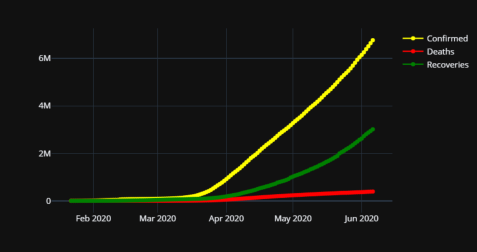
\includegraphics[scale=0.4]{images/world_wide.png}
	\caption{Number of cases around the world}
	\label{fig:world}
\end{figure}

%\section{Theory}
%
%

%\pagebreak

\section{Methods and models}

\subsection{Data}
The dataset used was the 2019 Novel Coronavirus Dataset operated by the
Johns Hopkins University Center for Systems Science and Engineering
(JHU CSSE).

It consist of 3 dataset each of Death, Confirmed, Recovered cases of 188
countries datewise. The number of date columns are 138 starting from 22
Jan,2020 to 8 June,2020.Out of this about 85\% are used as training data
and the rest used as testing and validating data. So the model would be
predictingnext 15\% data value.

The prediction would not be made on a specific country rather it will be
worldwide.

\begin{table}[!ht]
	\caption{World Dataset of Corona virus spread with confirmed, death,
	and recovery rates}
	\centering
	\resizebox{\columnwidth}{1.5cm}{%
		\begin{tabular}{lrrrrrrrr}
			\toprule
			{} &     Confirmed &    Recoveries &         Deaths &
			Confirmed Change &  Recovery Rate &  Growth Rate & \\
			\midrule
			count &  1.390000e+02 &  1.390000e+02 &     139.000000 &        138.000000 &     139.000000 &   138.000000 \\
			mean  &  1.918547e+06 &  6.817390e+05 &  123264.726619 &      50666.268116 &       0.286331 &     0.076081 \\
			std   &  2.170725e+06 &  8.911273e+05 &  138597.907312 &      42526.463980 &       0.143922 &     0.117824 \\
			min   &  5.400000e+02 &  2.800000e+01 &      17.000000 &         89.000000 &       0.017598 &     0.005032 \\
			25\%   &  7.862450e+04 &  2.747150e+04 &    2703.000000 &       2957.500000 &       0.207790 &     0.021193 \\
			50\%   &  8.430870e+05 &  1.738930e+05 &   44056.000000 &      67738.000000 &       0.288055 &     0.032183 \\
			75\%   &  3.546736e+06 &  1.142438e+06 &  249918.000000 &      84446.500000 &       0.395898 &     0.085793 \\
			max   &  6.992485e+06 &  3.220219e+06 &  397840.000000 &     130518.000000 &       0.544809 &     0.951446 \\
			\bottomrule
		\end{tabular}}
	  \label{table:world_df}
\end{table}


%\pagebreak
\subsection{Evaluation Metrics}

To identify best model, it is necessary to put concentration on comparison of measures of
the algorithm’s performance. In this report, MAPE and Accuracy are used to
measure algorithm's performance-

\begin{enumerate}
	\item \textbf{Mean Absolute Percentage Error}: It is defined by
		the following formula:
		\begin{equation}\label{eqn1}
			%E = {mc^2}
			MAPE = \frac{100\%}{n} \sum \left \vert \frac{y-y\prime}{y}
			\right \vert
		\end{equation}

		Where y is true value and y' is predicted value.

	\item \textbf{Accuracy}: It is defined by the following formula:
		\begin{equation}\label{eqn2}
			Accuracy = (100 - MAPE)\%
		\end{equation}

\end{enumerate}


\subsection{Method}

The prediction of confirmed cases of COVID 19 Corona virus are obtained
using a Recurrent Neural Network method(LSTM) and Linear Regression.

Linear regression is a linear model, that assumes a linear relationship between the input variables
(x) and the single output variable (y).When there is a single input variable (x), the method
is referred to as simple linear regression.

A Recurrent Neural Network (RNN) is kind of neural network architecture that considers
both sequential and parallel information processing. Incorporating memory cells to neural
network; it is possible to simulate the operations similar to human brain.There are
alternatives from RNN depending on the gating units, such as Long Short Term Memory
(LSTM) RNN and Gated Recurrent Unit (GRU) RNN.Traditional RNN lacks of
considering context based prediction, which can be overcome by introducing Long short-
term memory (LSTM). LSTM has a good potential to regulate gradient flow and enable
better preservation of long-range dependencies \cite{bandyopadhyay2020machine}.


\begin{figure*}[!ht]
	  \centering
	  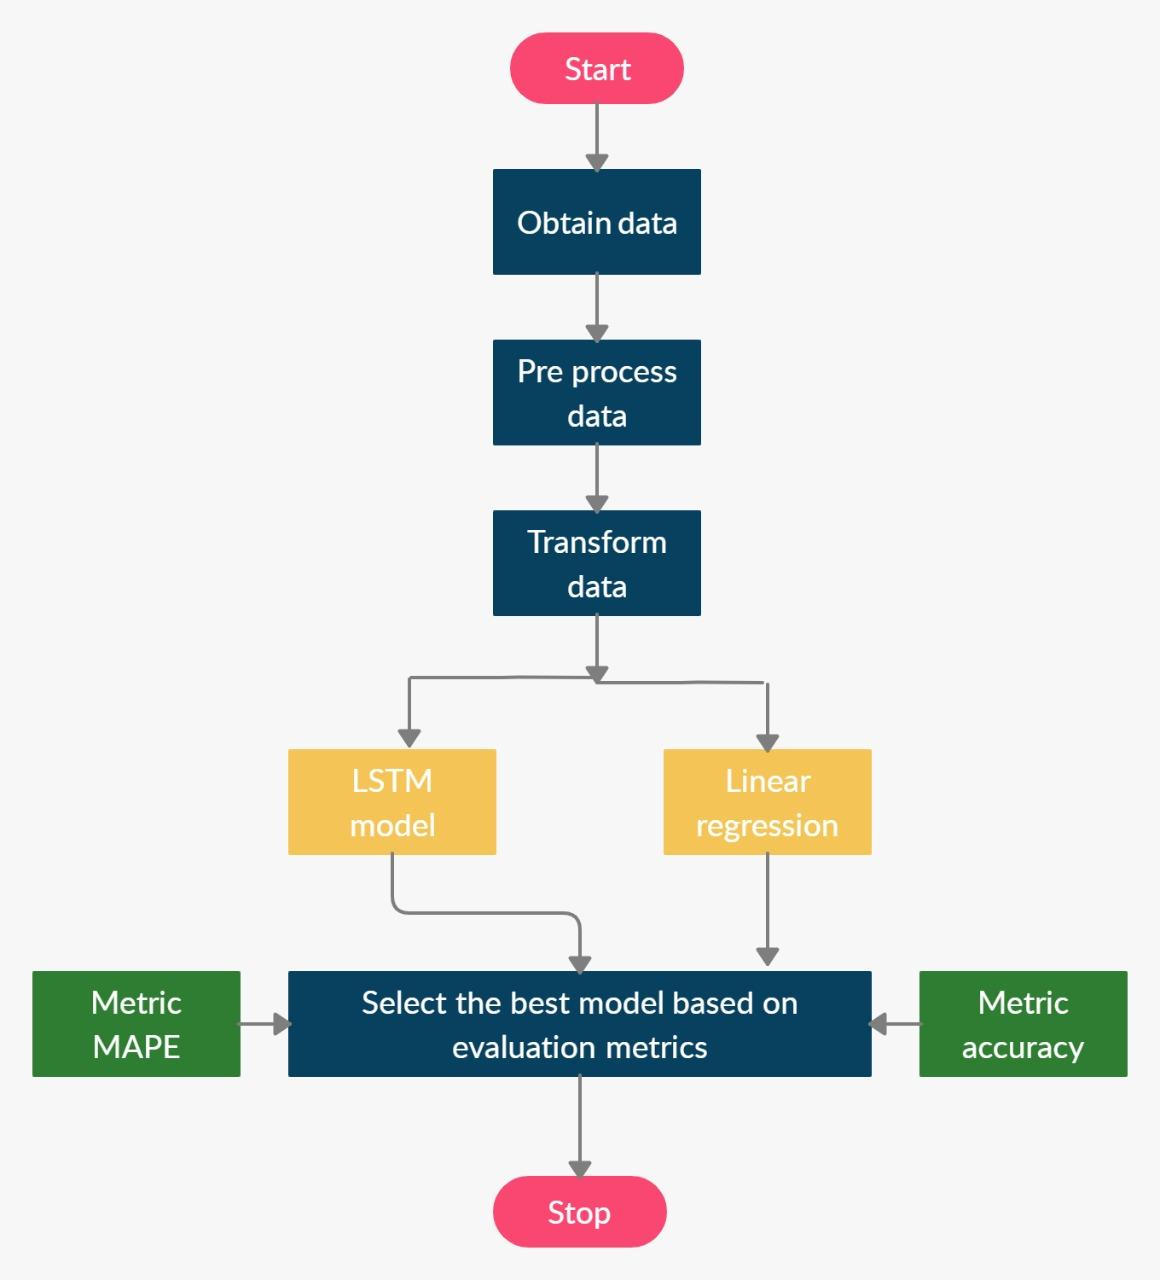
\includegraphics[height=9.5cm]{images/method.jpg}
	  \caption{Flowchar for proposed methodology}
	  \label{fig:method_flow}
\end{figure*}



The dataset used for predicting the value is taken from John Hopkin University which
contains cases form 22 January 2020 to 8 June,2020.Training and testing of both the models
is done on this dataset.It contains 138 date columns out of which 120 are used for training
and the rest 18days are used for testing data or for forecasting it.At first the data is preprocessed by converting the date columns into datetime object and also eliminate the
missing values. The preprocessed data is then transformed in the required shape to be put
into the model.The models are trained and the test data is predicted and prediction result
are quantified using performance measures metrics such as MAPE and
accuracy.The methodology performed for each of the step is shown in the figure
\ref{fig:method_flow} as show.


\textbf{Linear Regression}

Linear regression is used for prediction tasks.In a problem wuth one predicting value this
technique is used which tries to best fit the value to a linear line.This line can be used to
relate both the predicting and predicted value.When there is more than one value then the

In case of exponential relations, linear regression can not be directly used.
But after transformation to a linear expression, even exponential relations can
be predicted using linear regression. For example,
\begin{equation}
	y = \alpha e^{\beta x}
\end{equation}

Taking the log on both sides of the equation, we get:

\begin{equation}
	\ln y = \ln \alpha + \beta x
\end{equation}

This expression is of the form of a linear regression model:
\begin{equation}
	y\prime = \alpha \prime + \beta x
\end{equation}



\textbf{LSTM Model}

Long Short term memory is an recurrent neural network which is most effective for time
series prediction.The model used in this case is sequential.As the data was time series and
we needed to predict the best positive corona cases so this model was best for our study.The
model was build using tensorflow keras framework and the models performance was
evaluated on the mean absolute error percentage (MAPE) and accuracy metrics.
The proposed architecture of LSTM model is shown in the figure
\ref{fig:lstm_arch} as:

\begin{figure}[ht!]
	\centering
	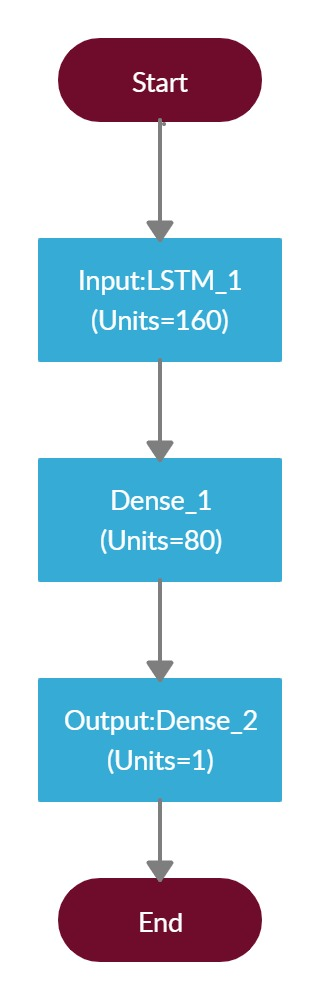
\includegraphics[scale=0.3]{images/lstm_mod.jpg}
	\caption{Architecture of LSTM model}
	\label{fig:lstm_arch}
\end{figure}

\newpage

\section{Experiment Result}

In LSTM model, LSTM layers use sequence of 50 nodes. A 2 layered structure followed by
a Dense Layer is used as LSTM model for verifying prediction result. The best
hyperparameters used is a batch size of 1.The prediction accuracy of the model
is shown in table \ref{table:lstm}


\begin{table}[ht!]
	\centering
	\caption{Accuracy and MAPE of LSTM model}
	\resizebox{5cm}{!}{
	\begin{tabular}{c c c}
		Model & Accuracy & MAPE \\
		LSTM model & 96.90\% & 3.092\%
	\end{tabular}}
	\label{table:lstm}
\end{table}

%\pagebreak
%\begin{figure}[ht!]
%	\centering
%	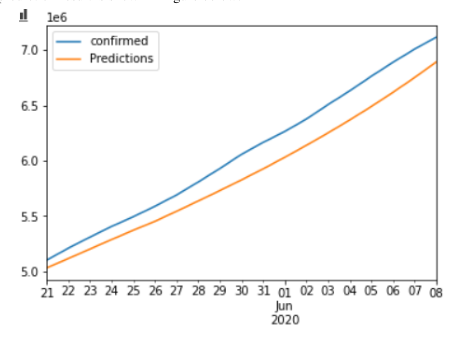
\includegraphics[scale=0.45]{images/lstm_graph.png}
%	\caption{Comparison of predicted and true value using LSTM model}
%	\label{fig:lstm_graph}
%\end{figure}
%\pagebreak

Linear regression was also applied on the time series data and the date columns were taken
as input and the 18 days data was predicted. The exponential fit of the model
was fit and the prediction accuracy of the model is shown in table
\ref{table:linear}

\begin{table}[ht!]
	\centering
	\caption{Accuracy and MAPE of regression model}
	\resizebox{5cm}{!}{
	\begin{tabular}{c c c}
		Model & Accuracy & MAPE \\
		Linear model & 93.57\% & 6.421\%
	\end{tabular}}
	\label{table:linear}
\end{table}

The prediction result of comparing the test data predicted data is show below:
\begin{figure}[ht!]
    \centering
    \subfloat[Comparison of predicted and true value using LSTM
	model]{{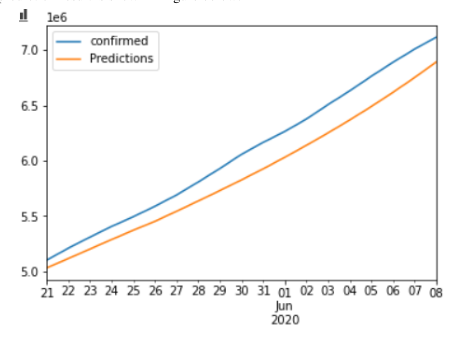
\includegraphics[scale=0.45]{images/lstm_graph.png} }}%
    \qquad
    \subfloat[Comparison of predicted and true value using Linear Regression
	model]{{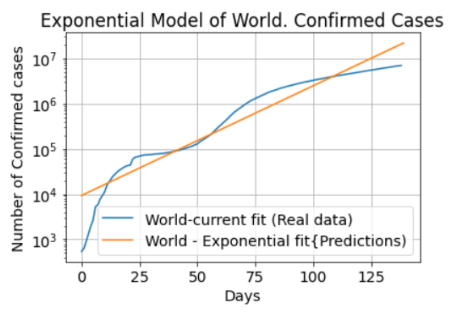
\includegraphics[scale=0.45]{images/linear_graph.png} }}%
    \caption{Results}%
    \label{fig:LinearandLstm}%
\end{figure}


%\begin{figure}[ht!]
%	\centering
%	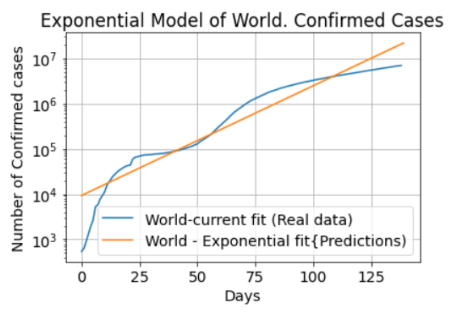
\includegraphics[scale=0.45]{images/linear_graph.png}
%	\caption{Comparison of predicted and true value using Linear Regression model}
%	\label{fig:linear_graph}
%\end{figure}

\pagebreak

\subsection{Comparing with other studies}
%
In \cite{hu2020artificial}, they used an multi-step forecasting system on
the population of china, and the estimated average errors are as show in
\ref{table:three}

\begin{table}[ht!]
	\centering
	\caption{Result \cite{hu2020artificial}: Method and Average Errors}
	\begin{tabular}{c c }
		Model & Error  \\
		6-Step & 1.64\% \\
		7-Step & 2.27\% \\
		8-Step & 2.14\% \\
		9-Step & 2.08\% \\
		10-Step & 0.73\%
	\end{tabular}
	\label{table:three}
\end{table}


In \cite{chimmula2020time}, LSTM netwoks are used to on Canadian population,
the reuslt are show is table \ref{table:four}

\begin{table}[ht!]
	\centering
	\caption{Results \cite{chimmula2020time}: Canadian Datasets}
	\begin{tabular}{c c c}
		Model & RMSE & Accuracy \\
		LSTM & 34.63 & 93.4\%

	\end{tabular}
	\label{table:four}
\end{table}


In \cite{bandyopadhyay2020machine}, an deep learning based approach is
proposed to campared the predicted forcasting value of LSTM and GRU model is
used the result are as show in table \ref{table:seven}:

\begin{table}[ht!]
	\centering
	\caption{Results \cite{chimmula2020time}: Canadian Datasets}
	\begin{tabular}{c c c}
		Model & RMSE & Accuracy \\
		LSTM & 53.35 & 76.6\% \\
		GRU & 30.95 & 76.9\% \\
		LSTM and GRU & 30.15 & 87\%

	\end{tabular}
	\label{table:seven}
\end{table}


\section{Conclusion and Future Scope}

The comparison between Regression and LSTM model signifies that LSTM provides a
comparatively better results in terms of prediction of confirmed data. This paper showcases a method that checks occurred cases of
COVID-19. However it could be made automated to train on the updated data
every week and see the predicted value. Also the model is trained only on confirmed cases
same could be done for both recovered and death cases and predicted values could be found.
The model shows only the worldwide cases however the dataset also provides country wise
statistics so it can be used by different country to forecast the future outcome of the
pandemic and take necessary preventive measures to be safe from this worldwide
pandemic.  In conclusion,
the data mining models could help policymakers and health managers to plan health care
resources and control the prevention of an epidemic outbreak. The availability of high-
quality and timely data in the early stages of the outbreak collaboration of
the researchers to analyze the data could have positive effects on health care
resource planning.

%\newpage


%\pagebreak
%\onecolumn
\printbibliography

\end{document}
